
%(BEGIN_QUESTION)
% Copyright 2007, Tony R. Kuphaldt, released under the Creative Commons Attribution License (v 1.0)
% This means you may do almost anything with this work of mine, so long as you give me proper credit

The wire coil of an electric solenoid valve has the ability to store energy in its magnetic field, just like any inductance ($U = {1 \over 2}LI^2$).  The potential for energy release from a solenoid coil igniting a hazardous atmosphere is particularly high when the coil is energized by DC: when the circuit is suddenly broken by the opening of a switch contact or by a loose wire connection, the rapid collapse of the solenoid's magnetic field induces a large voltage according to the formula $v = L{di \over dt}$.

One way to prevent this from occurring is to connect a {\it commutating diode} in parallel with the solenoid coil, as such:

$$\includegraphics[width=15.5cm]{i02472x01.eps}$$

In order to explain why this diode eliminates the problem of ``kickback voltage'' generated by the solenoid coil, you must be able to explain the behavior of an inductor as a {\it load} and as a {\it source}.  Determine both the direction of current through the inductor and the polarity of voltage across the inductor in the following two example circuits, and identify whether the inductor is acting as an energy source or as an energy load in both circuits.  Finally, explain how this relates to the solenoid circuit shown above:

$$\includegraphics[width=15.5cm]{i02472x02.eps}$$

\vskip 20pt \vbox{\hrule \hbox{\strut \vrule{} {\bf Suggestions for Socratic discussion} \vrule} \hrule}

\begin{itemize}
\item{} How would the circuit function if the commutating diode's polarity were reversed?
\item{} Explain why the addition of a commutating diode {\it slows down} the decay of the solenoid's magnetic field when the switch is opened.  In other words, explain why adding the diode to the circuit makes it so the solenoid valve takes longer to return to its ``normal'' (de-energized) state.
\end{itemize}

\underbar{file i02472}
%(END_QUESTION)





%(BEGIN_ANSWER)

The inductor acts as a {\it load} when the switch initially closes, and as a {\it source} when it opens.  The polarity reversal as the inductor transitions from load to source (with current maintaining the same direction) is what turns the diode on to provide a discharge current path for the inductor.

%(END_ANSWER)





%(BEGIN_NOTES)

$$\includegraphics[width=15.5cm]{i02472x03.eps}$$

\vskip 10pt

By clamping the inductor's ``source'' voltage to a mere 0.7 volts (approximate), the rate-of-change of current through the coil is clamped to a low value as well, following the formula:

$$v = L{di \over dt}$$

If $v$ is small, $di \over dt$ must likewise be small.  Since the coil's magnetic field is a direct function of current, this means the rate of magnetic field decay (${d \phi \over dt}$) must also be small.  For any given magnetic field strength, the presence of the commutating diode forces a longer decay time.

\vfil \eject

\noindent
{\bf Summary Quiz:}

Insert a protective diode into this circuit, to prevent the switch contacts from being destroyed by inductive ``kickback'' whenever the solenoid coil de-energizes:

$$\includegraphics[width=15.5cm]{i02472x04.eps}$$

\vfil \eject

\noindent
{\bf Summary Quiz:}

Sketch the direction(s) of all current(s) in this circuit at the moment when the pushbutton switch opens up:

$$\includegraphics[width=15.5cm]{i02472x01.eps}$$


%INDEX% Electronics review: inductor as source versus load
%INDEX% Safety, intrinsic: commutating diode for DC solenoid coils

%(END_NOTES)


